\documentclass[10pt]{beamer}
\usetheme[
%%% option passed to the outer theme
%    progressstyle=fixedCircCnt,   % fixedCircCnt, movingCircCnt (moving is deault)
  ]{Feather}
  
% If you want to change the colors of the various elements in the theme, edit and uncomment the following lines

% Change the bar colors:
%\setbeamercolor{Feather}{fg=red!20,bg=red}

% Change the color of the structural elements:
%\setbeamercolor{structure}{fg=red}

% Change the frame title text color:
%\setbeamercolor{frametitle}{fg=blue}

% Change the normal text color background:
%\setbeamercolor{normal text}{fg=black,bg=gray!10}

%-------------------------------------------------------
% INCLUDE PACKAGES
%-------------------------------------------------------
\usepackage{subfig}
\usepackage[utf8]{inputenc}
\usepackage[english, spanish]{babel}
\usepackage[T1]{fontenc}
\usepackage{helvet}
\setbeamertemplate{caption}[numbered]
\setbeamertemplate{frametitle continuation}{} %continuation of frames
\bibstyle

% Another Packages

\usepackage{array}
\usepackage{float}
\usepackage{multirow}
\usepackage{amssymb}
\usepackage{graphicx}

% Tikz

\usepackage{tikz}
\usetikzlibrary{mindmap}
\definecolor{myblue}{HTML}{020364}
\usetikzlibrary{shapes,arrows,matrix,decorations.pathreplacing,shapes.geometric,positioning}  
% Gantt
\usepackage{pgfgantt}
\usepackage{adjustbox} %Ajustar a la página

% Items

\usepackage{enumitem}
\usepackage{amsfonts}

%videos

%\usepackage{media9}
\usepackage{multimedia}

% No numbering in references

%\newcommand{\backupbegin}{
%   \newcounter{framenumberappendix}
%   \setcounter{framenumberappendix}{\value{framenumber}}
%}
%\newcommand{\backupend}{
%   \addtocounter{framenumberappendix}{-\value{framenumber}}
%   \addtocounter{framenumber}{\value{framenumberappendix}} 
%}

%-------------------------------------------------------
% DEFFINING AND REDEFINING COMMANDS
%-------------------------------------------------------

% colored hyperlinks
\newcommand{\chref}[2]{
  \href{#1}{{\usebeamercolor[bg]{Feather}#2}}
}

%-------------------------------------------------------
% INFORMATION IN THE TITLE PAGE
%-------------------------------------------------------

\title[Passive Dynamic System for Energy Returning on Transtibial Prosthesis] % [] is optional - is placed on the bottom of the sidebar on every slide
{ % is placed on the title page
      \textbf{Passive Dynamic System for Energy Returning on Transtibial Prosthesis}
}

\author[Edwin N. Prieto]
{      Nikolay Prieto PhD(c). \\
      {\ttfamily enprietop@unal.edu.co}
}

\institute[]
{
      Doctorate in Engineering - Mechanics and Mechatronics Department\\
      School of Engineering\\
      Universidad Nacional de Colombia Bogotá\\
  
  %there must be an empty line above this line - otherwise some unwanted space is added between the university and the country (I do not know why;( )
}

\date{\today}

%-------------------------------------------------------
% THE BODY OF THE PRESENTATION
%-------------------------------------------------------

\begin{document}

%-------------------------------------------------------
% THE TITLEPAGE
%-------------------------------------------------------

{\BiOM% % this is the name of the PDF file for the background
\begin{frame}[plain,noframenumbering] % the plain option removes the header from the title page, noframenumbering removes the numbering of this frame only
  \titlepage % call the title page information from above
\end{frame}}


\begin{frame}[noframenumbering]{Outline}{}
\tableofcontents[
sectionstyle=show/show,
subsectionstyle=hide/hide/hide,
] 
\end{frame}

\AtBeginSection[]{

  \frame<beamer>[noframenumbering]{ 

    \frametitle{Outline}   

    \tableofcontents[
currentsection,
sectionstyle=show/shaded,
subsectionstyle=hide/hide/hide
] 
  }
}

\section{Motivation}
\begin{frame}{Recent Advances in Commercial Prosthesis}

\begin{figure}
\begin{centering}
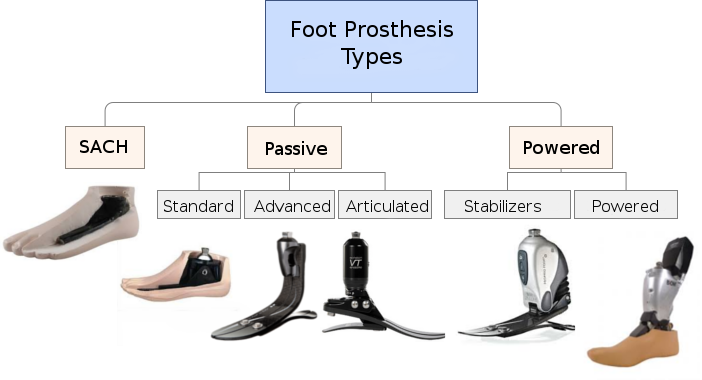
\includegraphics[scale=0.38]{Feathergraphics/GeneracionesprotesisEng}
\par\end{centering}
\caption{{\footnotesize{}Commercial prosthesis classes grouping. Adapted from Cherelle \emph{et al.} \cite{Cherelle2014a}} }

\end{figure}

\end{frame}

\begin{frame}{Energy Returning Principle}

\begin{figure}
\begin{centering}
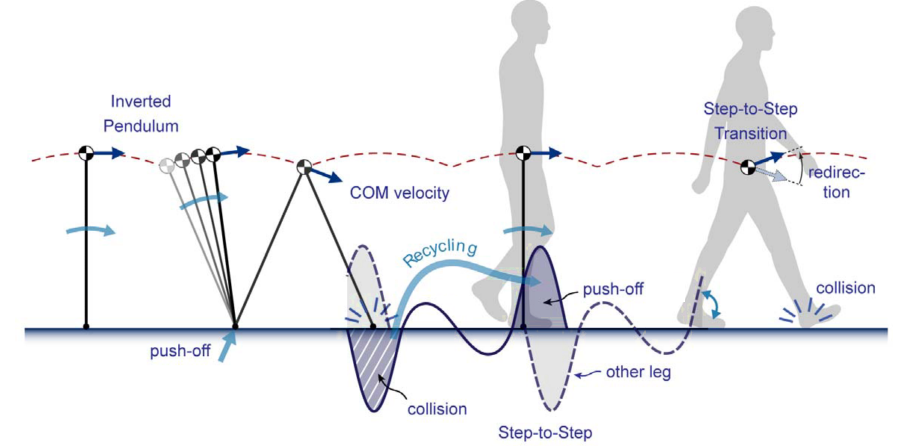
\includegraphics[scale=0.30]{Feathergraphics/RecycledEng}
\par\end{centering}

{\footnotesize \caption{\label{fig:Representaci} The leg in stance behaves similar to an inverted pendulum, supporting the body CoM until the other leg contacts the ground and mechanical energy is dissipated, then the vector velocity of the CoM is redirected. Figure modified from Collins and Kuo\cite{Collins2010}.}}

\end{figure}

\end{frame}



\begin{frame}{Principles of Prosthetic Feet}
\begin{alertblock}{}

\begin{itemize}
\item {Stiffness/flexibility.}
\item {Damping.}
\item {Roll-Over characteristics.}
\item {Active push-off in late stance phase.}
\item {Toe clearance during swing phase}
\end{itemize}
\end{alertblock}
\end{frame}

\begin{frame}{The Ankle Dynamic Joint Stiffness (DJS)}

\begin{figure}[h]
\begin{center}
\centerline{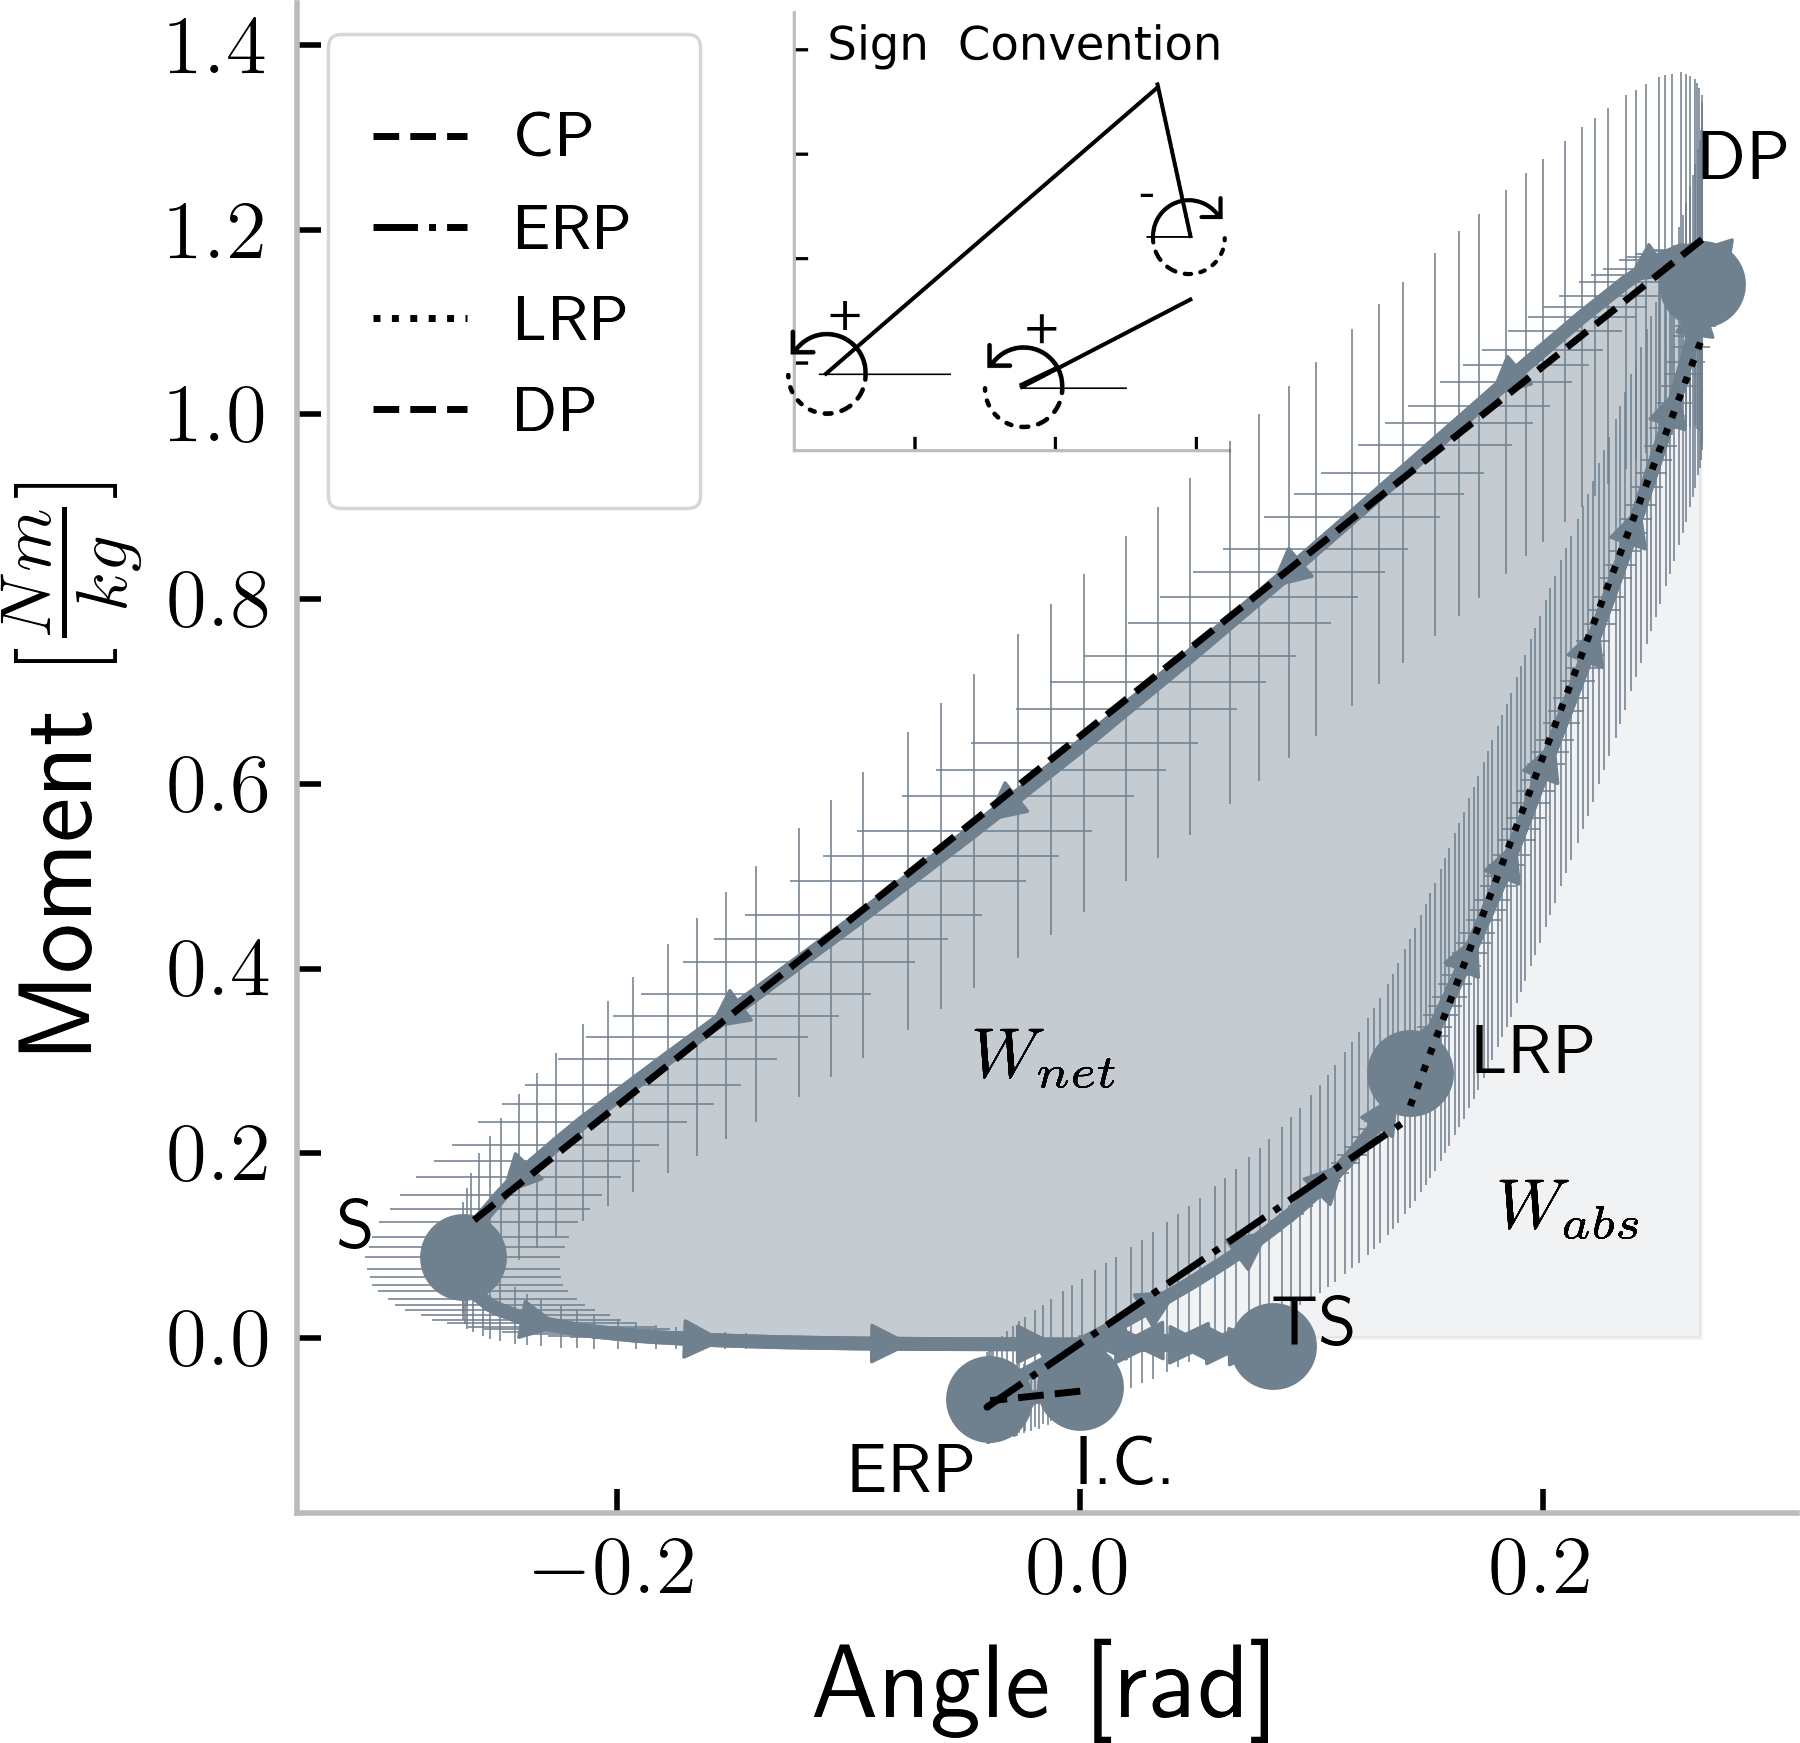
\includegraphics[scale=0.60]{Feathergraphics/general_conventions_QS.png}}
\caption{{\footnotesize Description of the Ankle DJS characteristics. Turning points represented as initiating: Contact (I.C), Early Response Phase (ERP), Late Response Phase (LRP), Descending Phase (DP), Swing (S) and Terminal Swing (TS). Regression fits: Controlled Plantar-flexion (CP), ERP, LRP and DP. Ankle DJS direction, mechanical net work ($W_{net}$), absorbed work ($W_{abs}$) and SD are shown on each DJS plot.}}
\label{fig:conventions}
\end{center}
\end{figure}

\end{frame}

%----------------------------------------------------------------
\section{Problem statement}

\subsection{Research Question and Objectives}

\subsection{Reseach Question}
\begin{frame}{Problem Statements}

\begin{block}{Research Question}

Which mechanical design variables for passive ankle-foot prosthesis, will generate the optimal quasi-stiffness trajectory \--- at different gait speeds and/or intentions \--- in order to generate the maximum positive work as possible?

More specifically, under the assumption that the in the optimal dynamic response of the foot prosthesis is the closest one provided by the missing ankle, what is the relative contribution of the each of the design parameters (thickness, size and shape) in such dynamic response? 

\end{block}
\end{frame}

\begin{frame}{Problem Statements}

\begin{block}{Hypothesis}

A passive dynamic system characterized by the optimal Design Variables within a passive ankle-foot prosthesis, configured to store energy at initial contact of the early stance phase, will be able to return \--- in a controlled manner \---  the maximum stored energy after dorsi-flexion phase in comparison with recent ESR prosthesis.

\end{block}
\end{frame}

\section{Objectives}

\subsection{Objectives}
\begin{frame}{Objectives}

\begin{alertblock}{General Objective}

To suggest an ankle-foot prosthesis being able to generate - through a passive dynamic system - the positive work needed for pushing-off after dual-flexion phase, taking advantage of the lost energy at the initial contact phase in gait.

\end{alertblock}
\end{frame}


\subsection{Specific Objectives}
\begin{frame}{Objectives}

\begin{exampleblock}{Specific Objectives}

\begin{enumerate}

\item To identify biomechanical parameters and the work-loop slope of ESR prosthesis users and non-amputees aiming to obtain the ankle quasi-stiffness in both cases.

\item To develop an \textit{in-silico} physical dynamic model of the ankle-foot prosthesis capable of storing energy (during initial contact until late dual-flexion phase), and returning it at dorsi-flexion phase in a controlled manner through the passive dynamic system.

\item To determine the most influenced design variables in the dynamic model for an ankle foot prosthesis.

\item To apply an optimization process in order to find the optimal positive work generated after dual-flexion phase. 

\end{enumerate}
\end{exampleblock}
\end{frame}

\section{The ankle DJS analysis for amputees}

\subsection{The proposed Algorithm}

\begin{frame}{The algorithm workflow}

\begin{figure}
\centerline{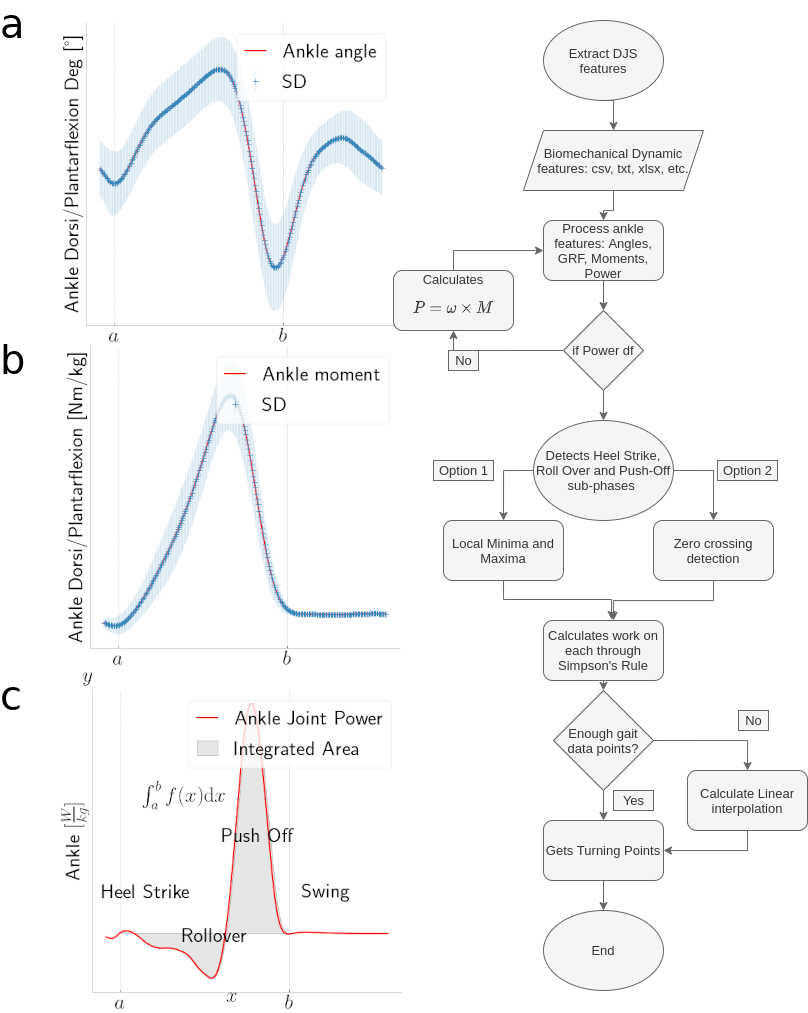
\includegraphics[scale=0.16]{Feathergraphics/flowchart_plus_plots.png}}
\caption{\label{fig:extract_flowchart} {\scriptsize (left) Ankle angle, moment and power subplots for a healthy subject at free speed. (right) General flowchart about the extraction of the features from an external dataset to process further for the ankle DJS characterization.}}
\end{figure}
\end{frame}

\subsection{Ipsilateral and contralateral limb.}

\begin{frame}{Transfemoral Amputee DJS Behavior}
\begin{footnotesize}
\begin{figure}[h]
\begin{center}
\centerline{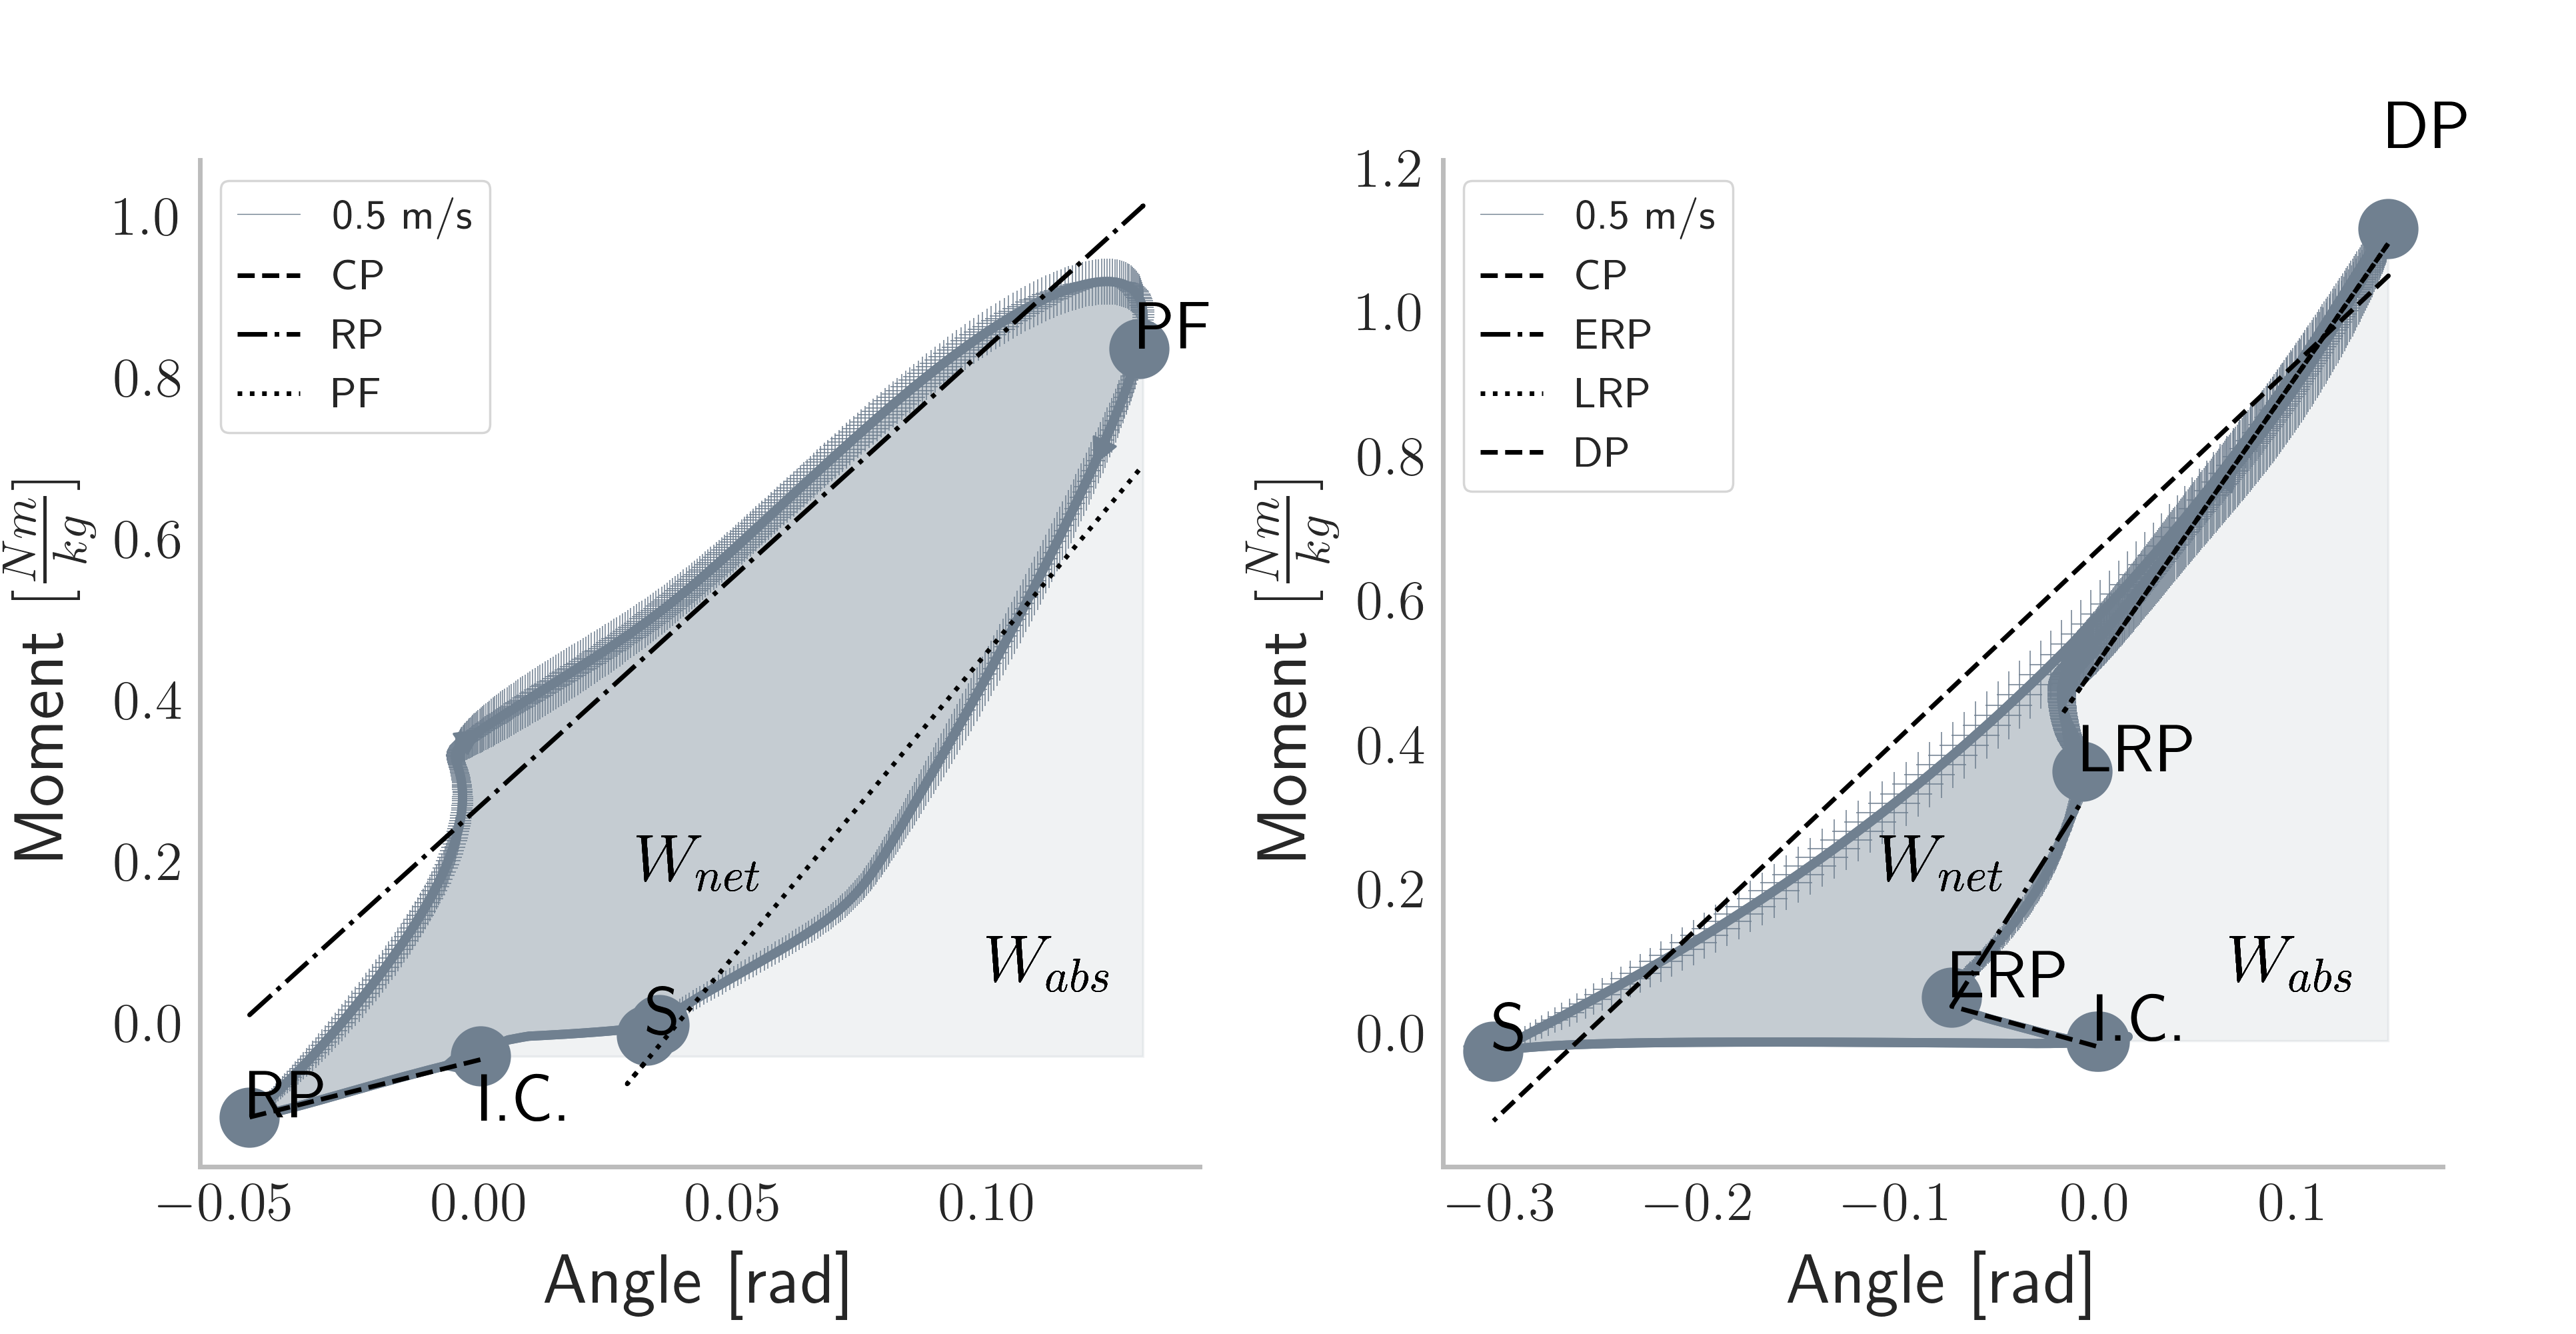
\includegraphics[scale=0.5]{Feathergraphics/amputee_convention.png}}
\caption{Description of the Ankle DJS characteristics for amputees in ipsilateral and contralateral limb. Turning points represented as initiating: Contact (I.C), Response Phase (RP), Plantar-flexion phase (PF) and, Swing (S) for ipsilateral. Regression fits: Controlled Plantar-flexion (CP), RP, PF. Ankle DJS direction, mechanical net work ($W_{net}$), absorbed work ($W_{abs}$). In contralateral, the convention remains as indicated in Fig. \ref{fig:conventions}}
\label{fig:conventions_amp}
\end{center}
\end{figure}
\end{footnotesize}
\end{frame}

\begin{frame}{Brand new prostheses DJS.}
\begin{footnotesize}
\begin{figure}
\centerline{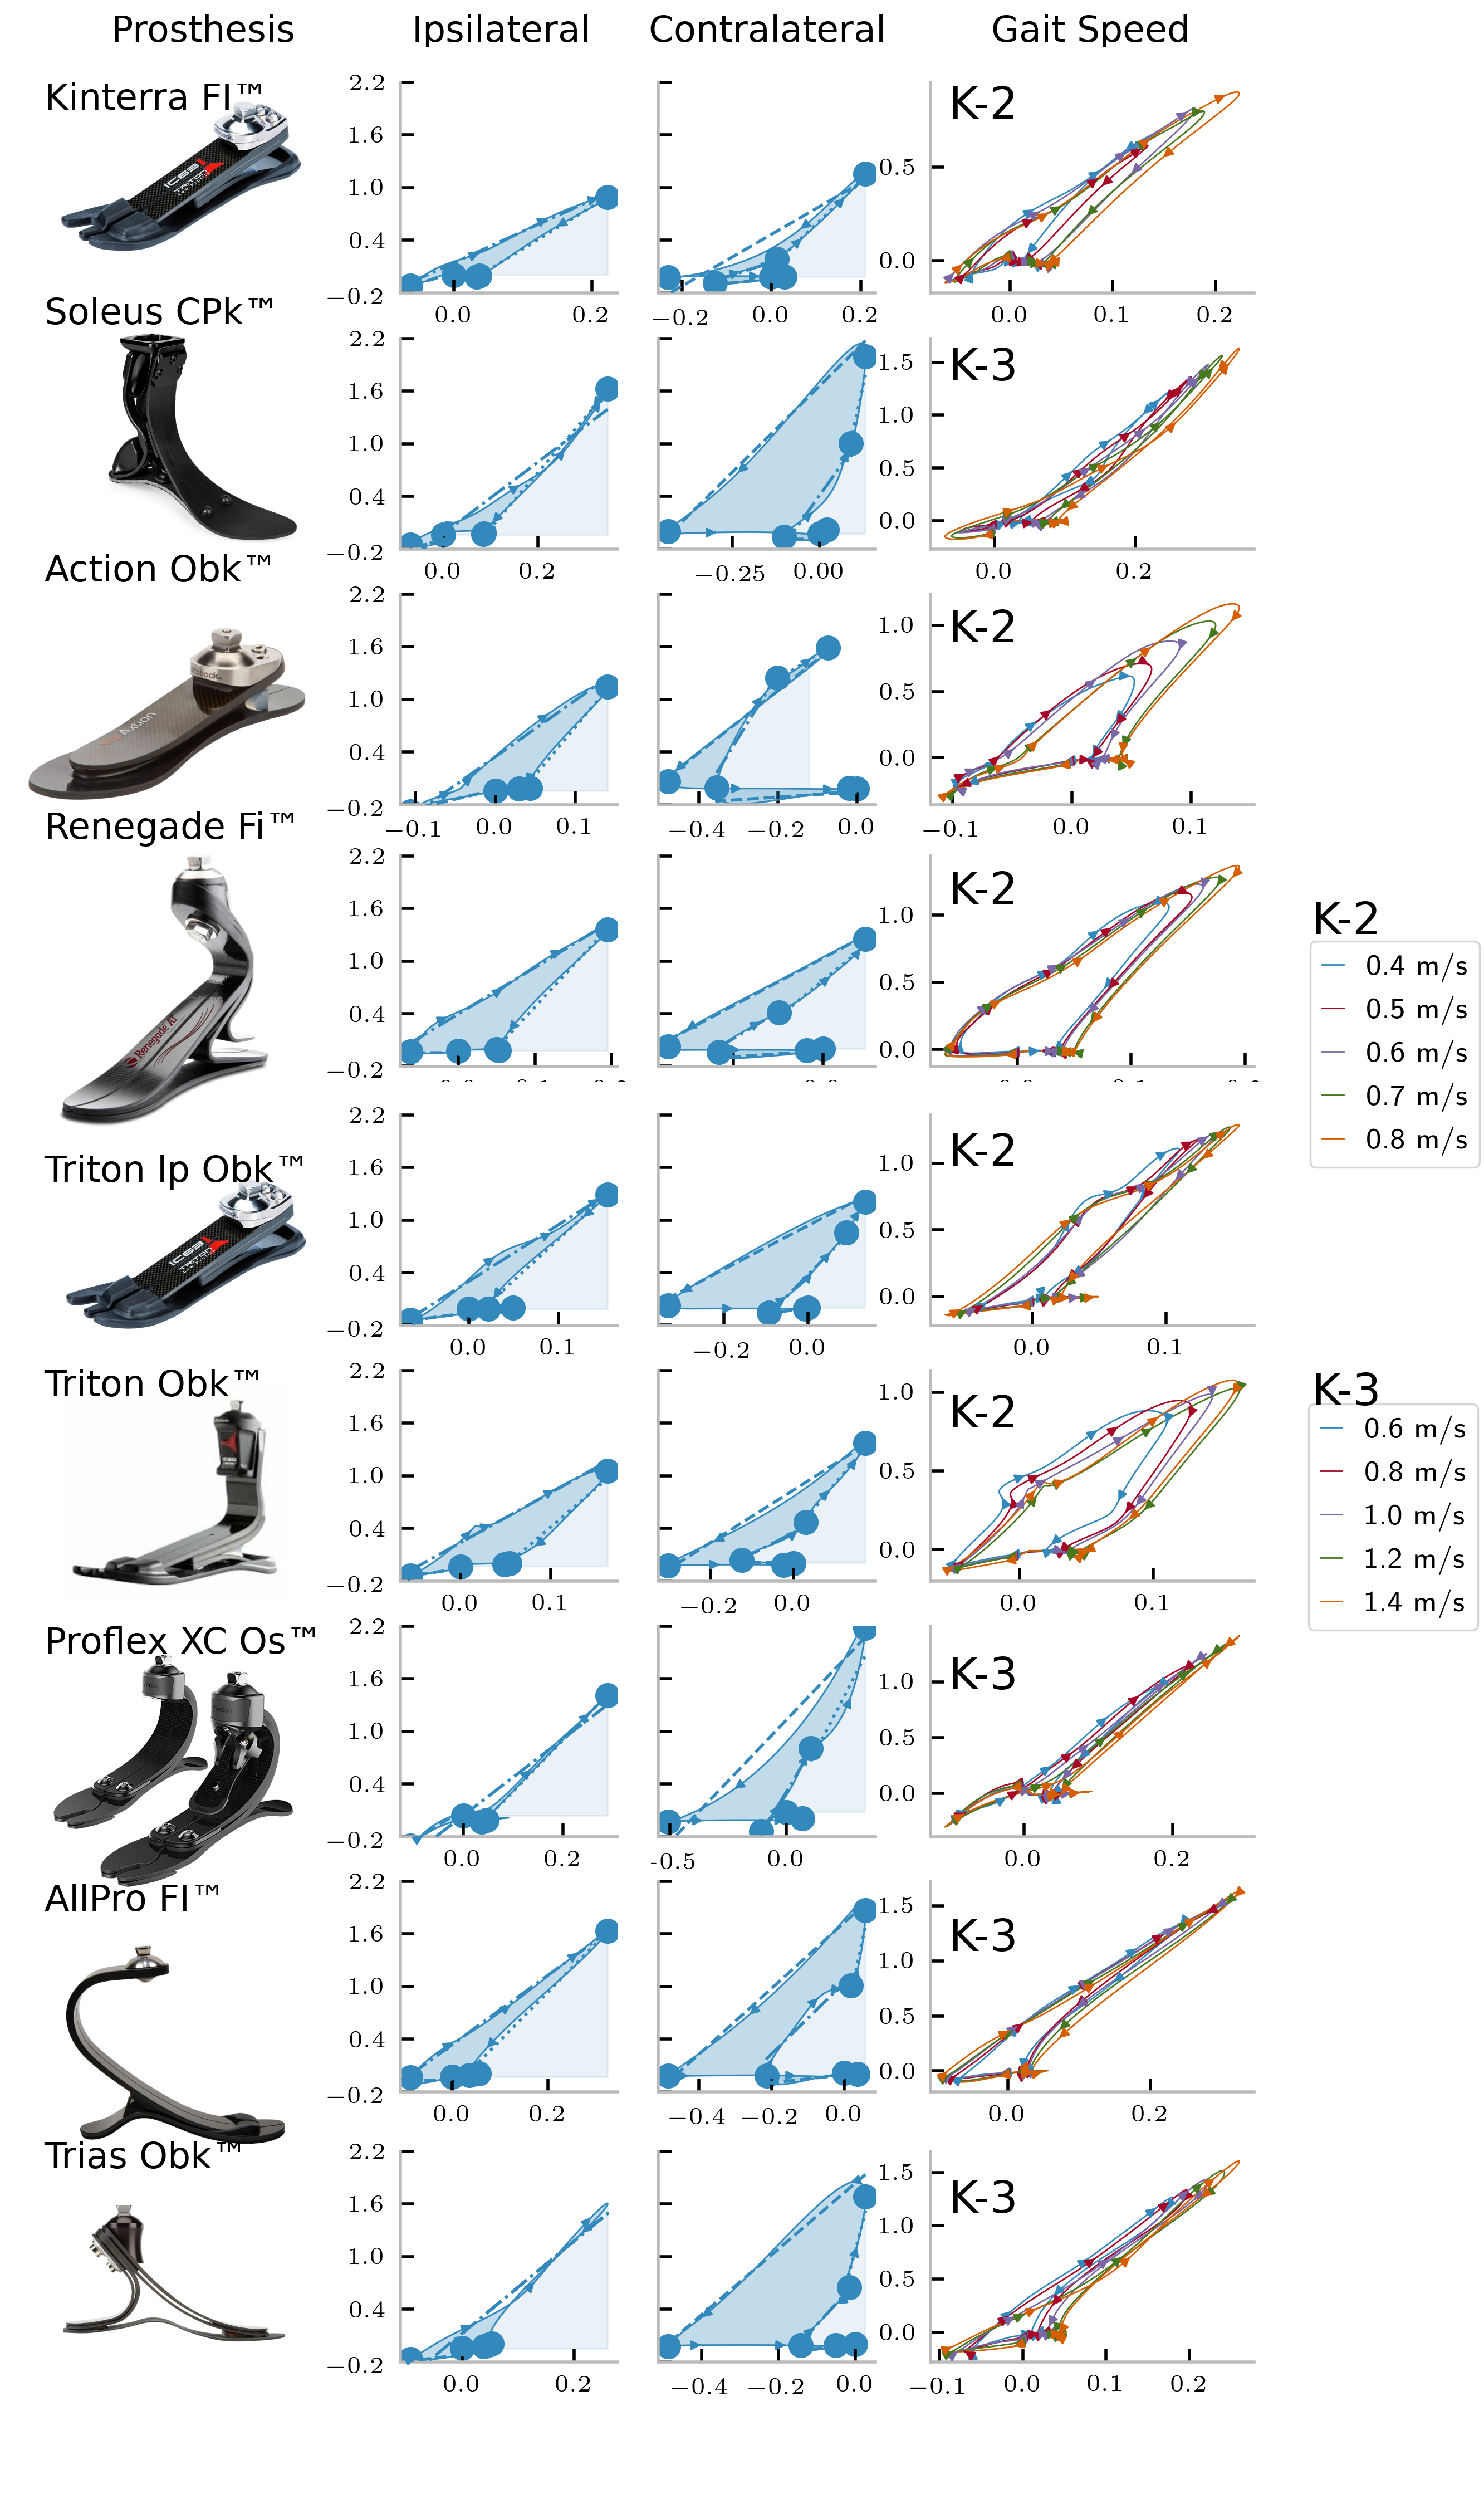
\includegraphics[scale=0.28]{Feathergraphics/prosthesisDJScomparison.png}}
\caption{\label{fig:benchmark} Benchmarks of recent ankle foot prosthesis available in the market and their ankle DJS characterization.}
\end{figure} 
\end{footnotesize}
\end{frame}

\section{The Global Sensitivity Analysis for an AF prosthesis model.}

\begin{frame}{The Dynamic Ankle Foot Model}
\begin{figure}
\centerline{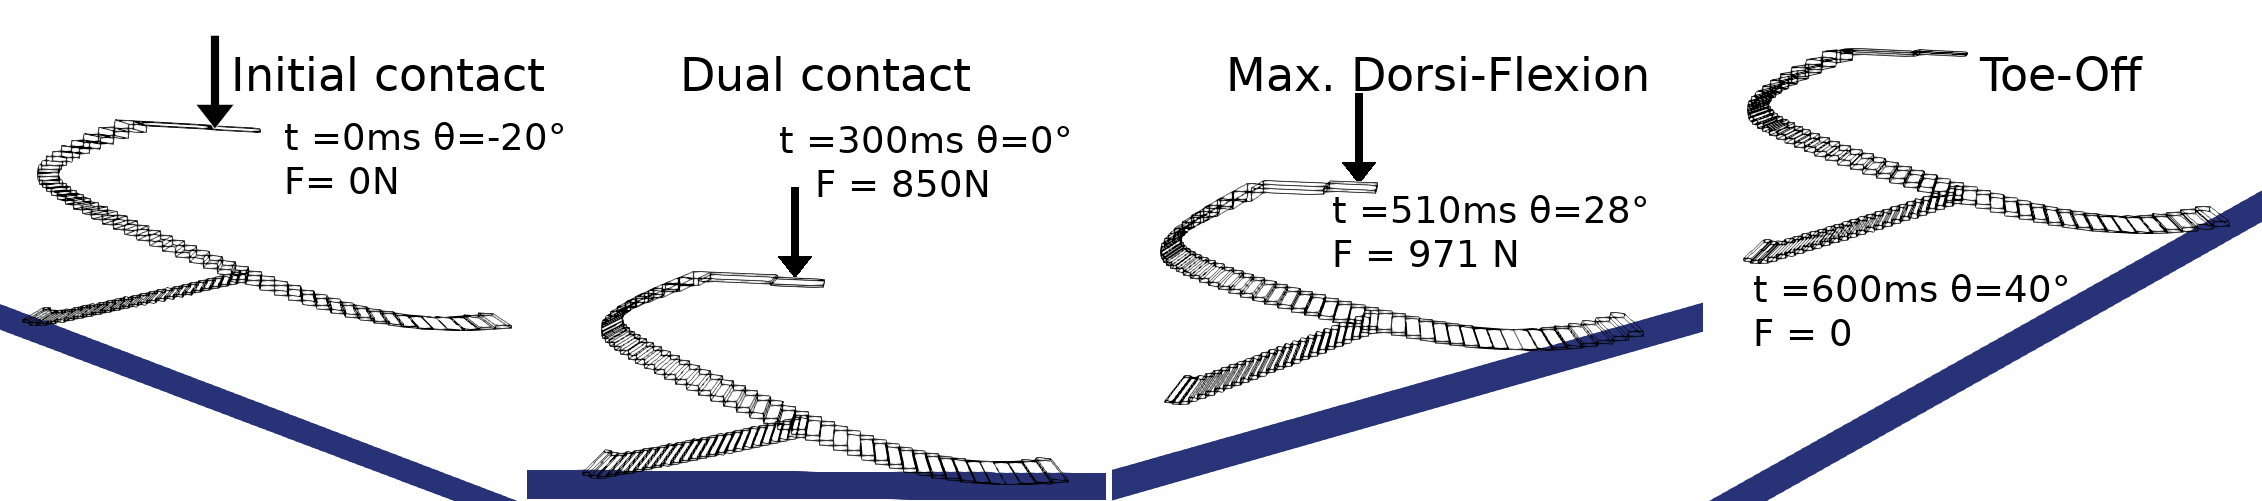
\includegraphics[scale=0.5]{Feathergraphics/Dynamic_path.png}}
\caption{\label{fig:Dynamic_foot} Dynamic process of the simulation. The two bonded laminates have elastic material properties. We set a force equivalent to the ISO 22675 along all the stance phase. Adittionally, the platform was set as a rigid body with a prescribed angular velocity so that the degrees established in the tables fit the needed position.}
\end{figure}
\end{frame}

\begin{frame}{General Boundary Conditions}
\begin{figure}
\centerline{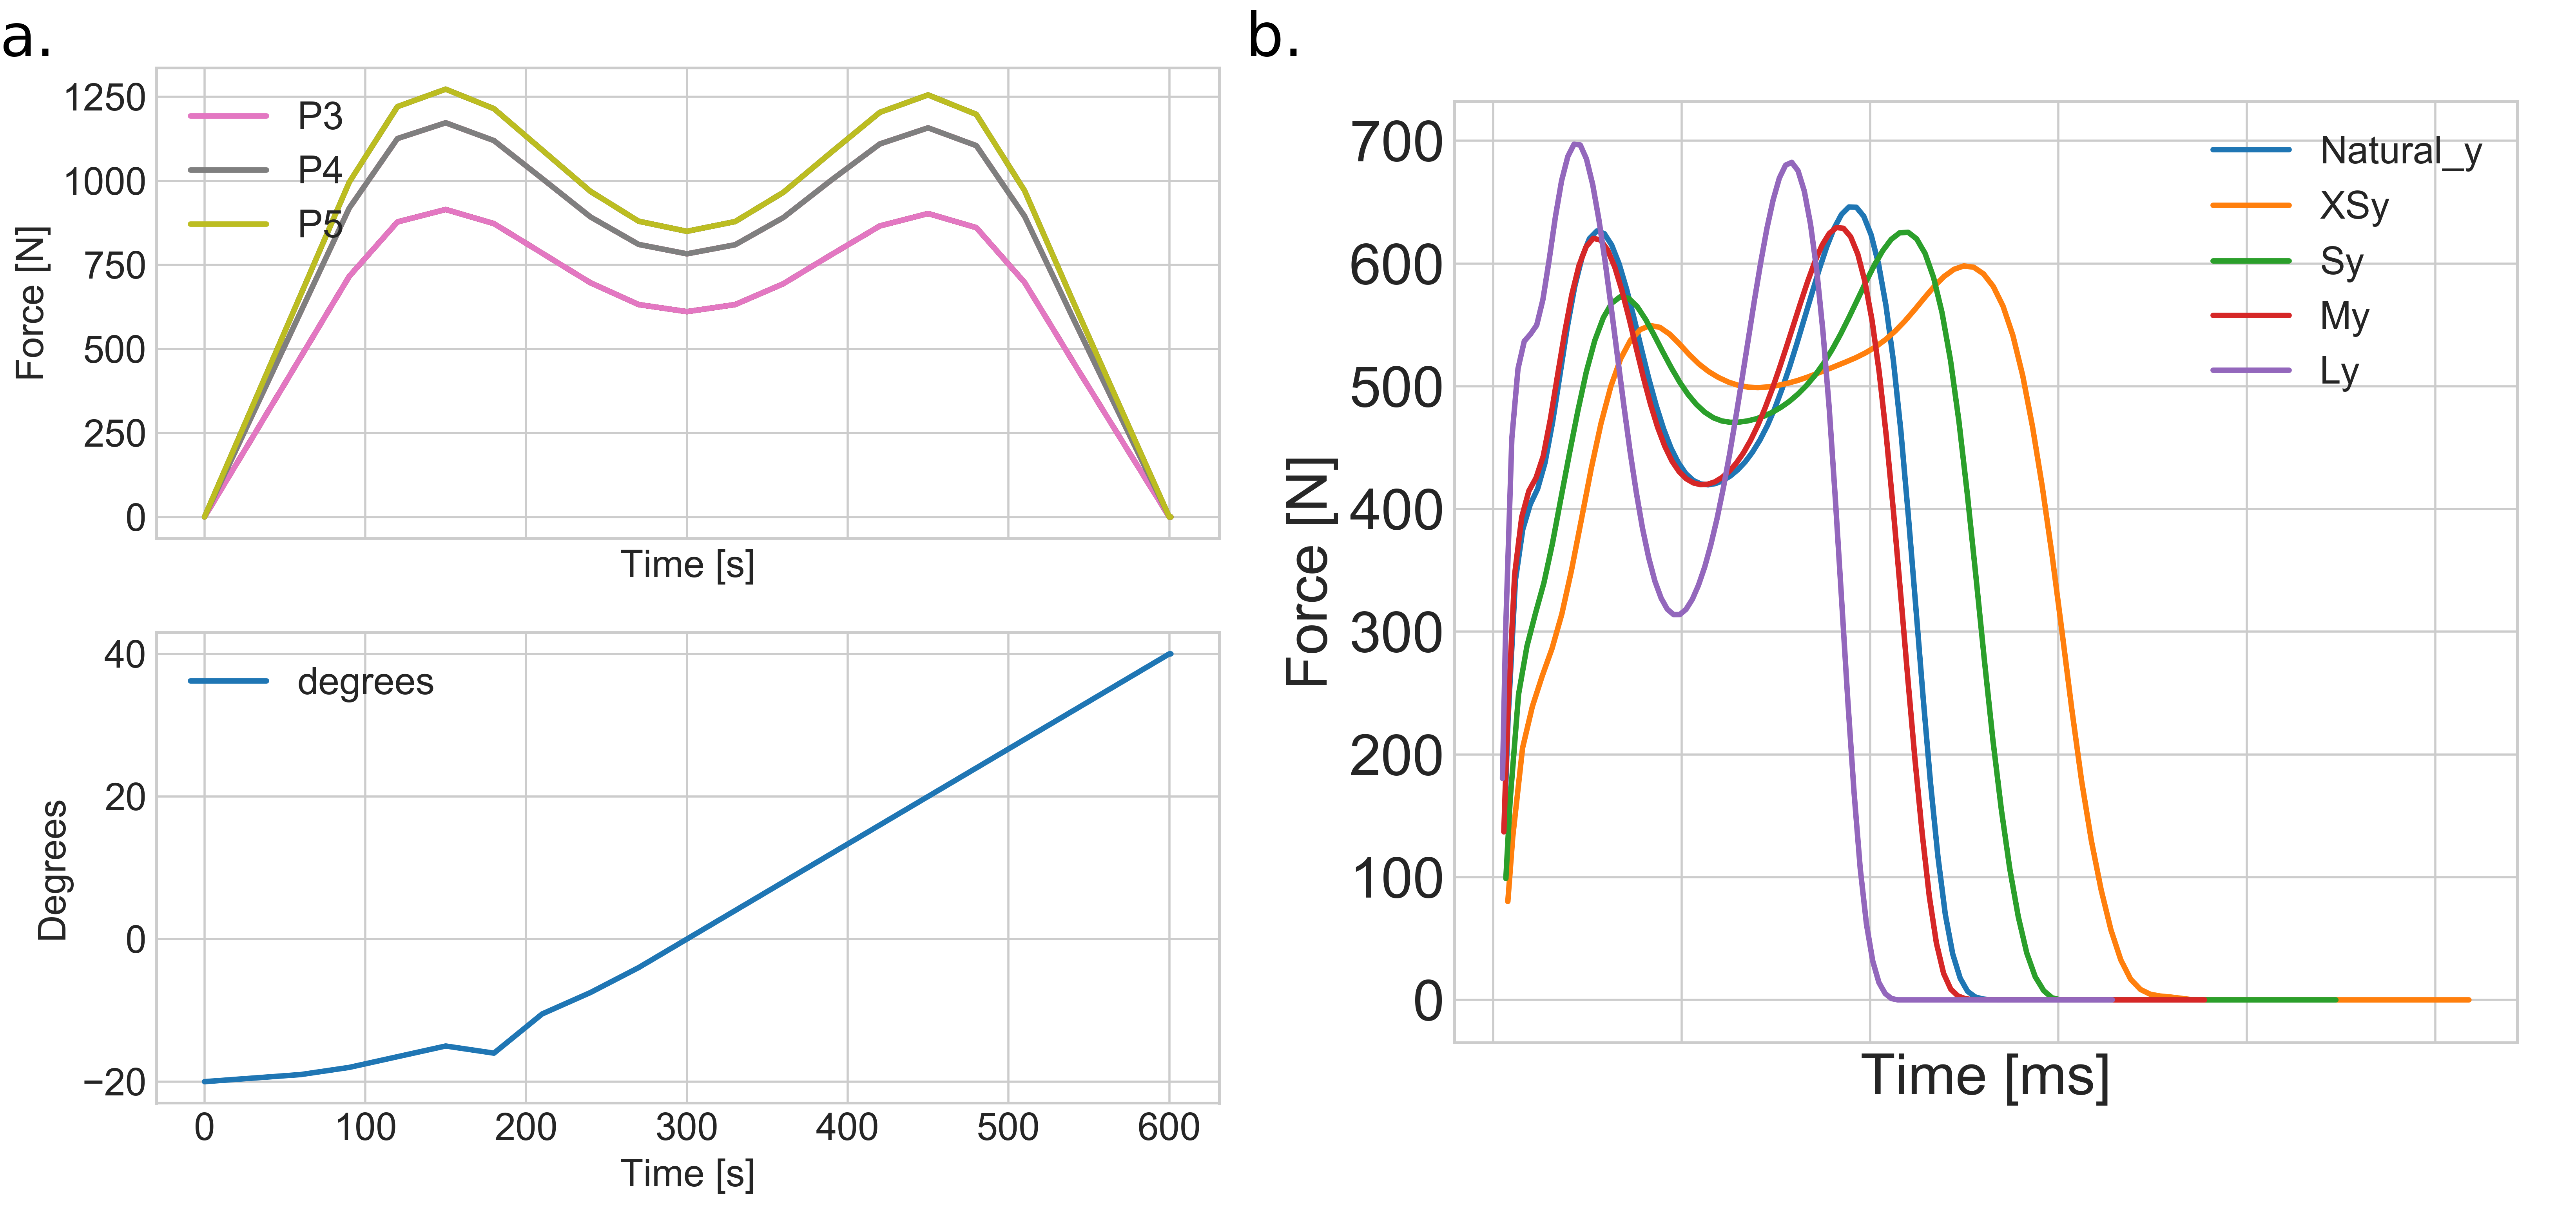
\includegraphics[scale=0.33]{Feathergraphics/combinedGRFISO_Real.png}}
\caption{\textbf{(a.)}\label{fig:ISO_GRF} Dynamic Input forces and platform angle according to \cite{ISO22675}. There are three levels of forces during the stance phase, in which P5 is the most difficult test and P3 is the easiest. \textbf{(b.)} Average GRF at different gait speed; from young adults. Data extracted from \cite{Bovi2011a}}
\end{figure}
\end{frame}


\begin{frame}{General Diagram of the Design Space.}
\begin{footnotesize}
\begin{figure}
\centerline{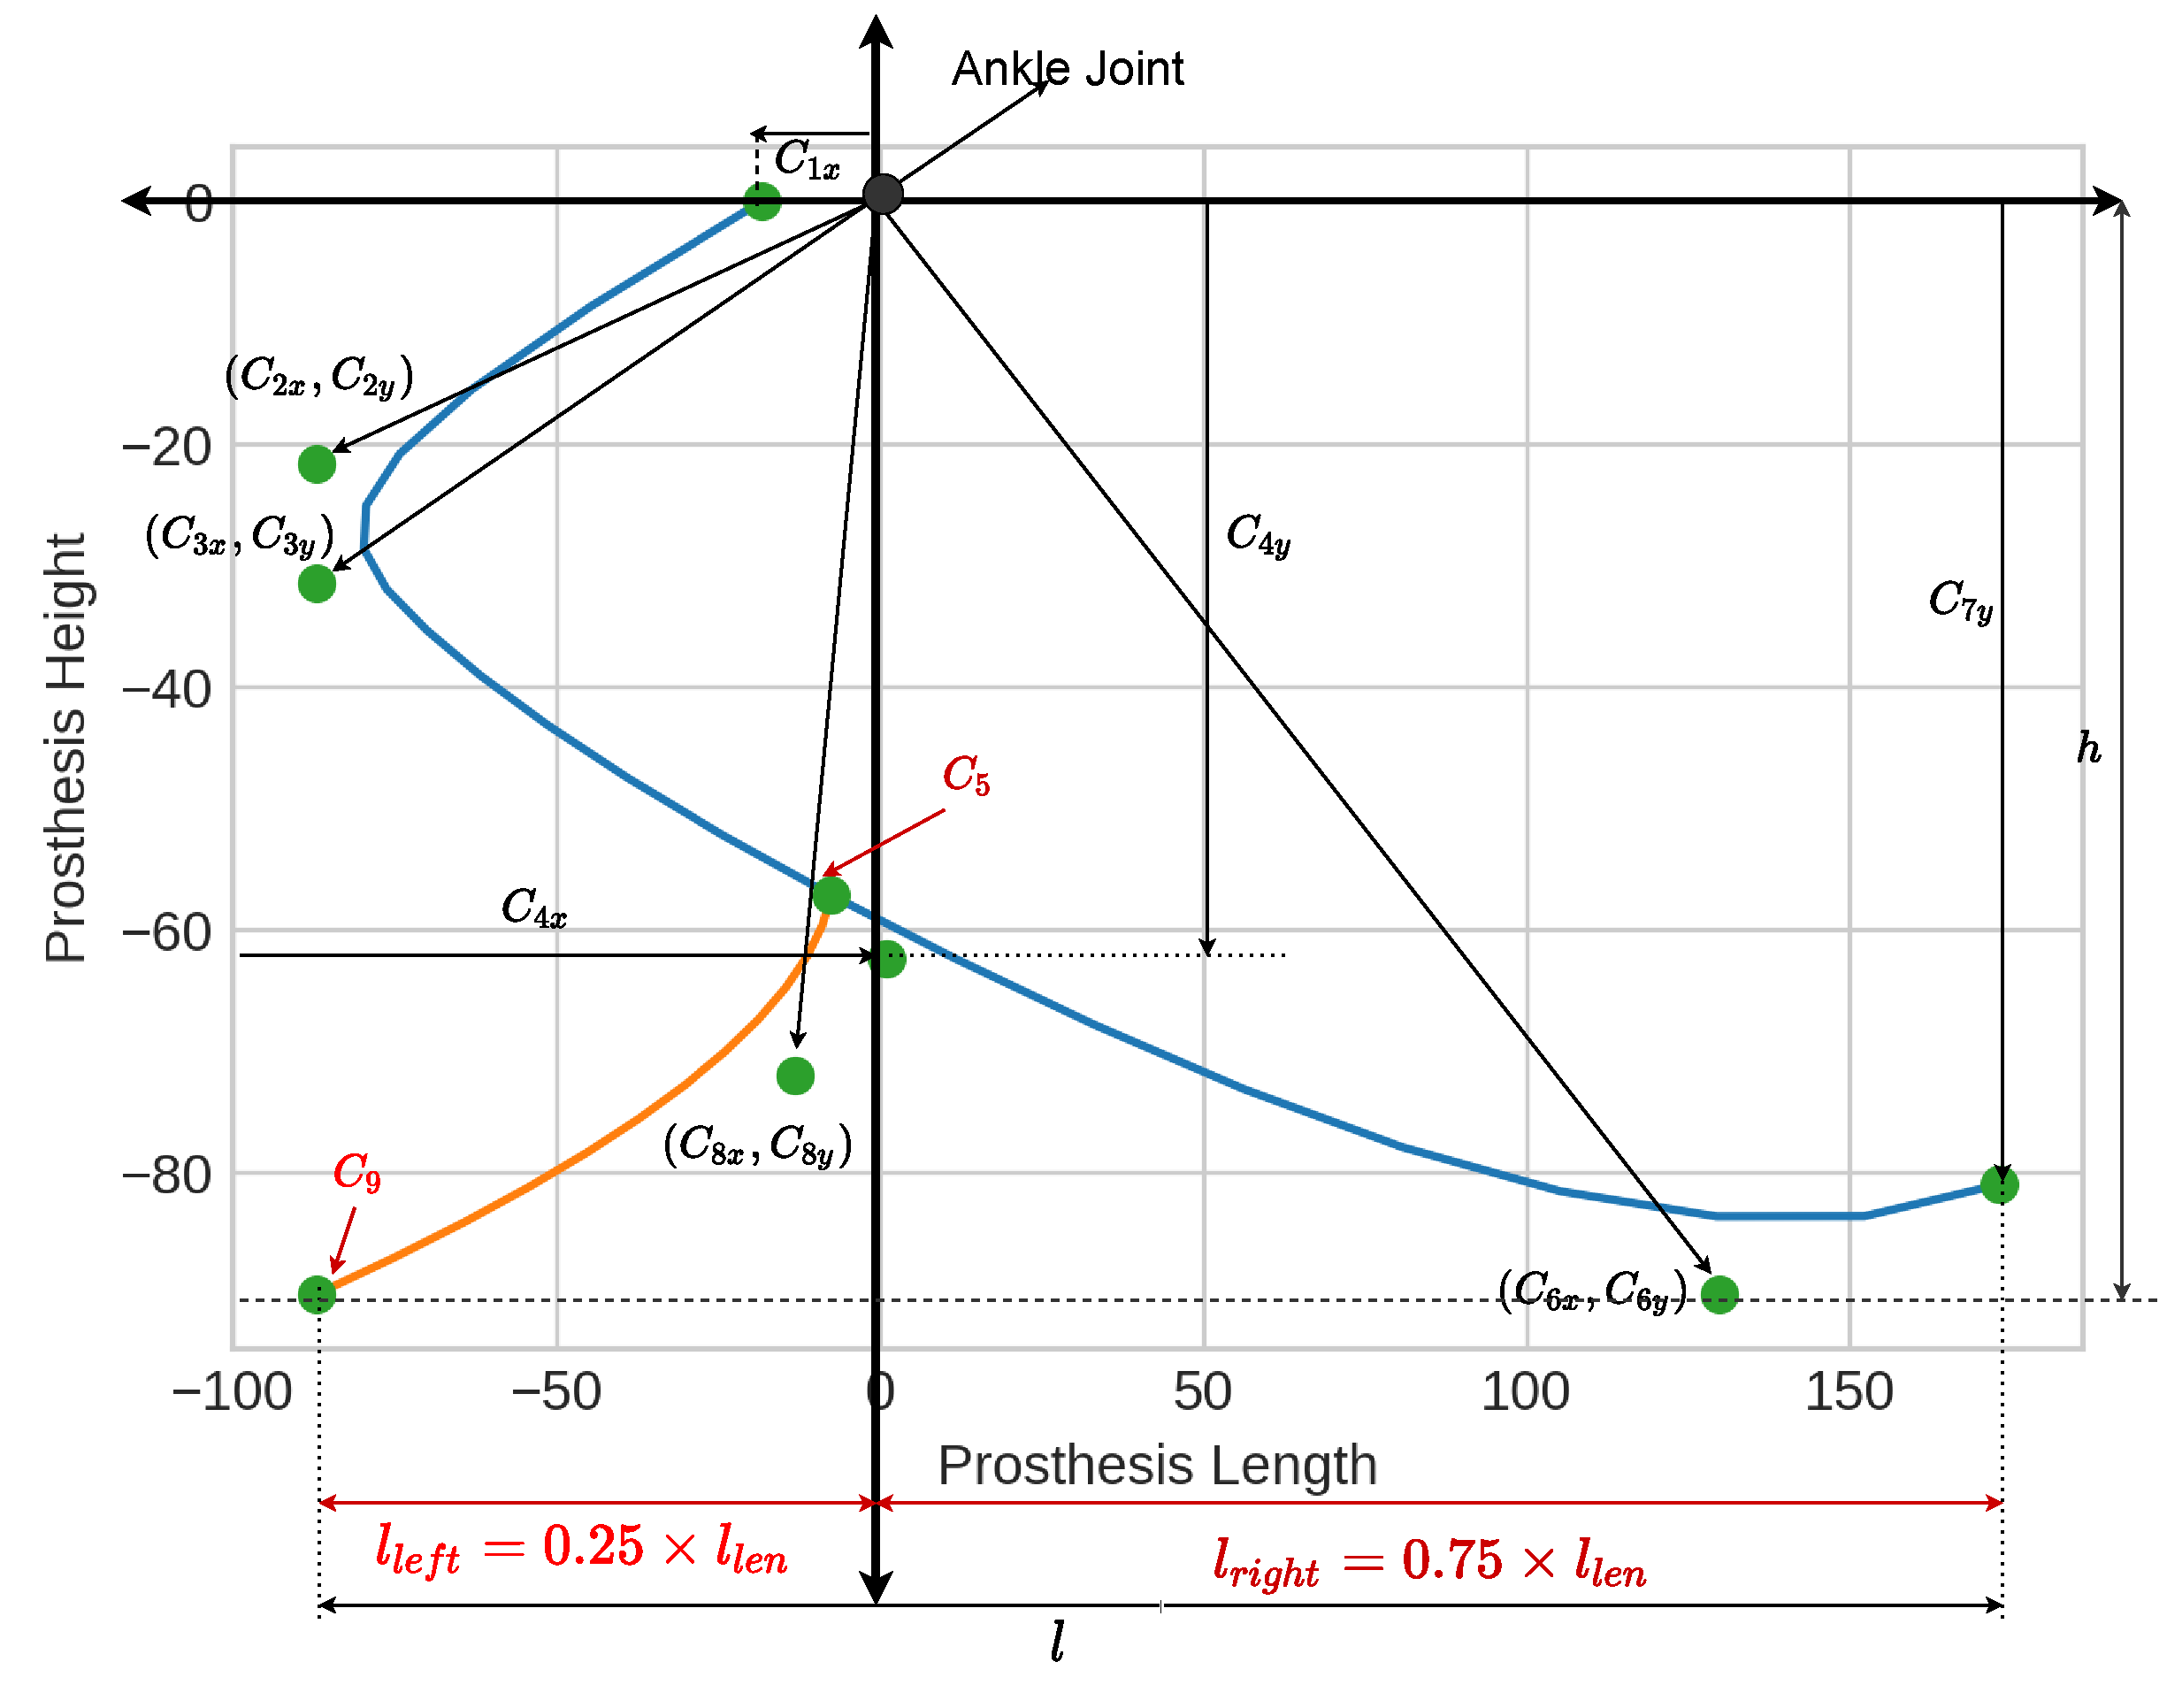
\includegraphics[scale=0.20]{Feathergraphics/ControlPointsDiagram.pdf}}
\caption{parametrization of the ankle-foot. The shape is controlled by the control points $(C_{nx}, C_{ny})$, foot length $l_{len}$ and height $h$. The red labels are fixed parameters \label{fig:shape_variables}.}
\end{figure}
\end{footnotesize}
\end{frame}

\begin{frame}{The Output variables}
\begin{footnotesize}
\begin{figure}
\centerline{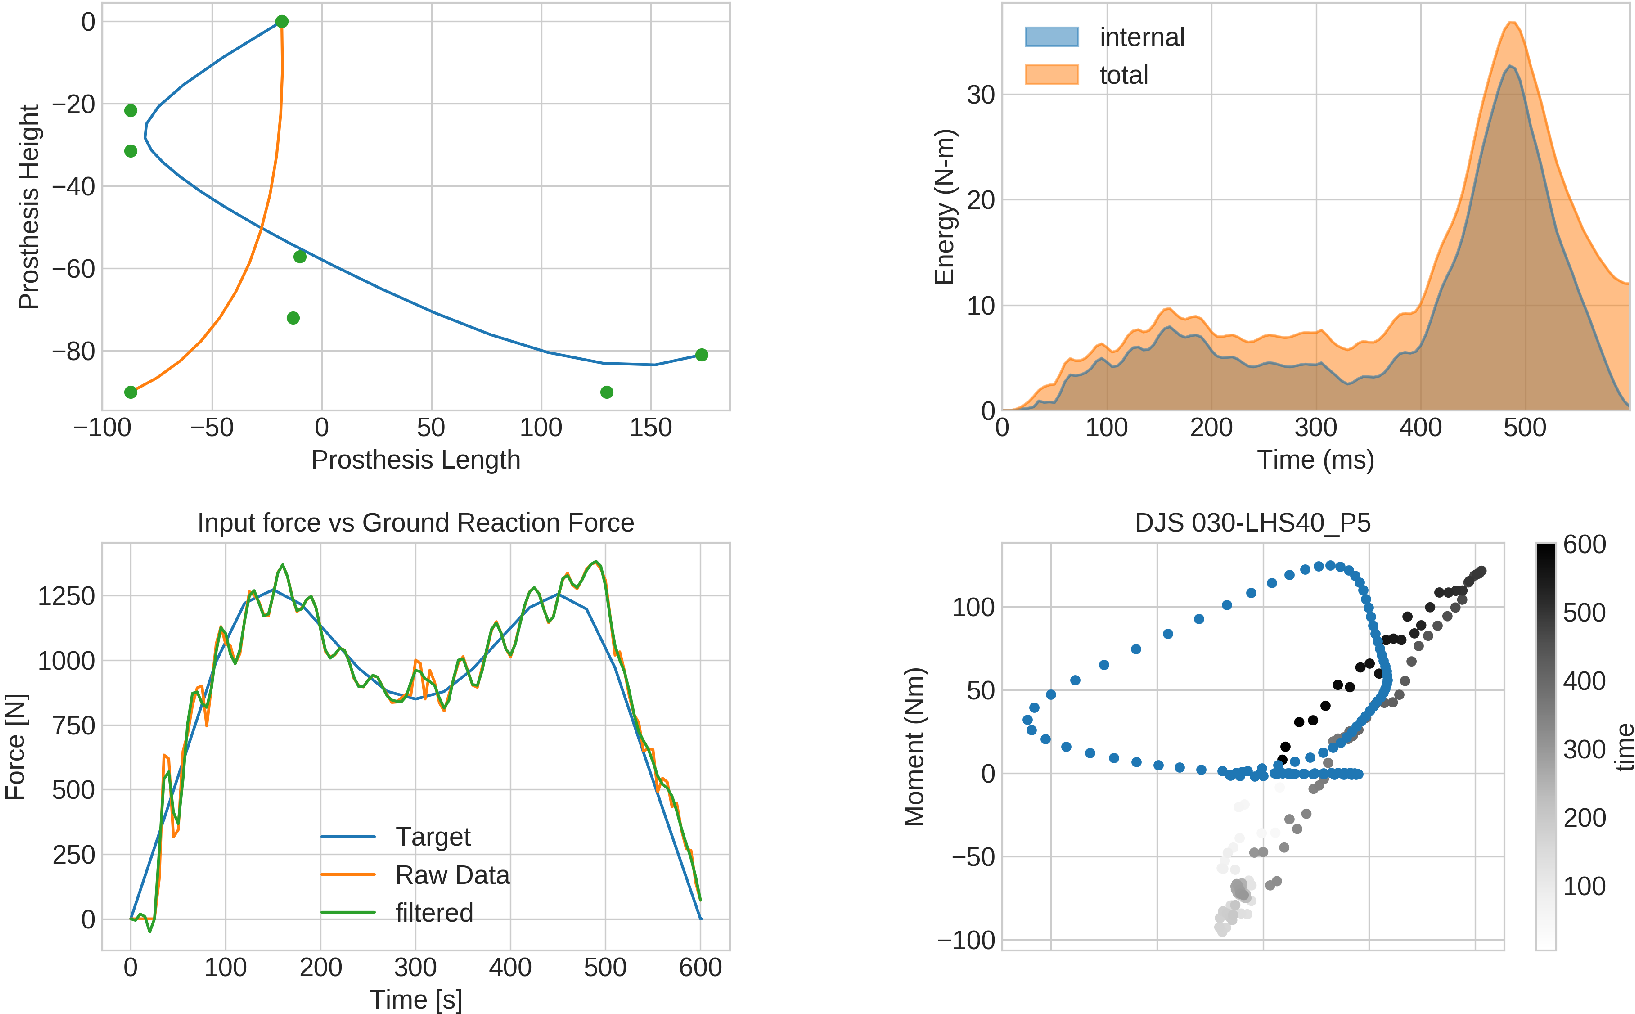
\includegraphics[scale=0.6]{Feathergraphics/complete_viz.png}}
\caption{\label{fig:Best-all-together} Example of general visualization of the output results according to the mechanical variables set in one simulation: (top left) sagittal shape proposed, (top right) strain energy, (Bottom left) GRF output and, (bottom right) ankle DJS. Bottom figures show the target reference and the respective output by the simulation.}
\end{figure}
\end{footnotesize}
\end{frame}


\begin{frame}{The sensitivity estimates}
\begin{footnotesize}
\begin{figure}
\centerline{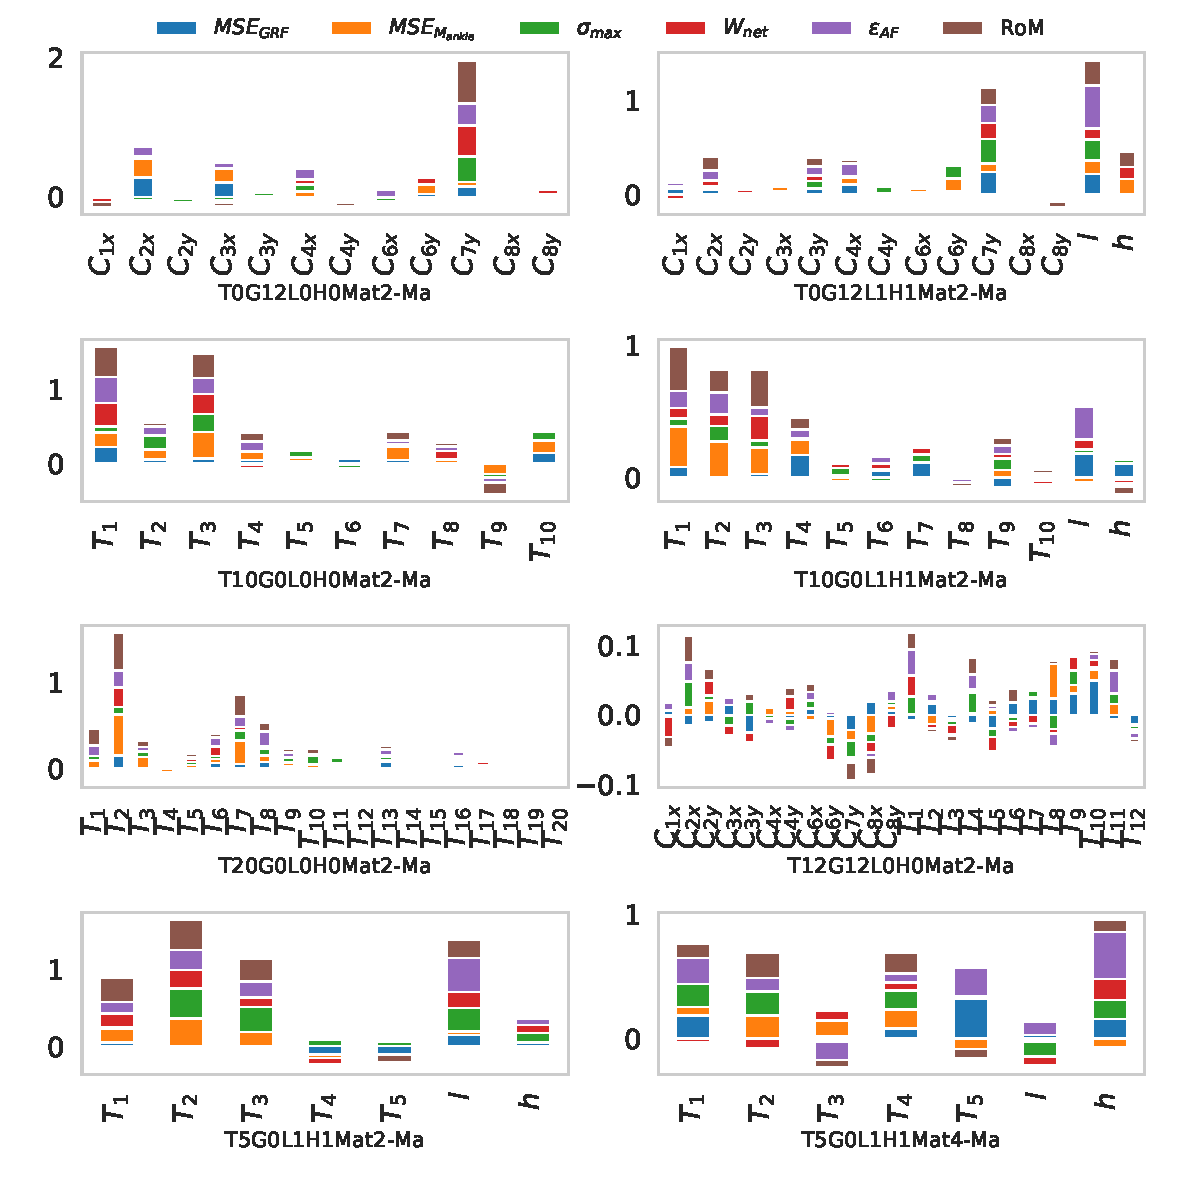
\includegraphics[scale=0.3]{Feathergraphics/SensitivityestimatesFEAmodel.pdf}}
\caption{Visualization of the Sensitivity estimates accumulation on each experiment. The $y$ axis represents the sensitivity magnitude accumulation in outputs.\label{fig:sensitivity_LHS}.}
\end{figure}
\end{footnotesize}
\end{frame}

\begin{frame}{The pair plot of the SA}
\begin{footnotesize}
\begin{figure}
\centerline{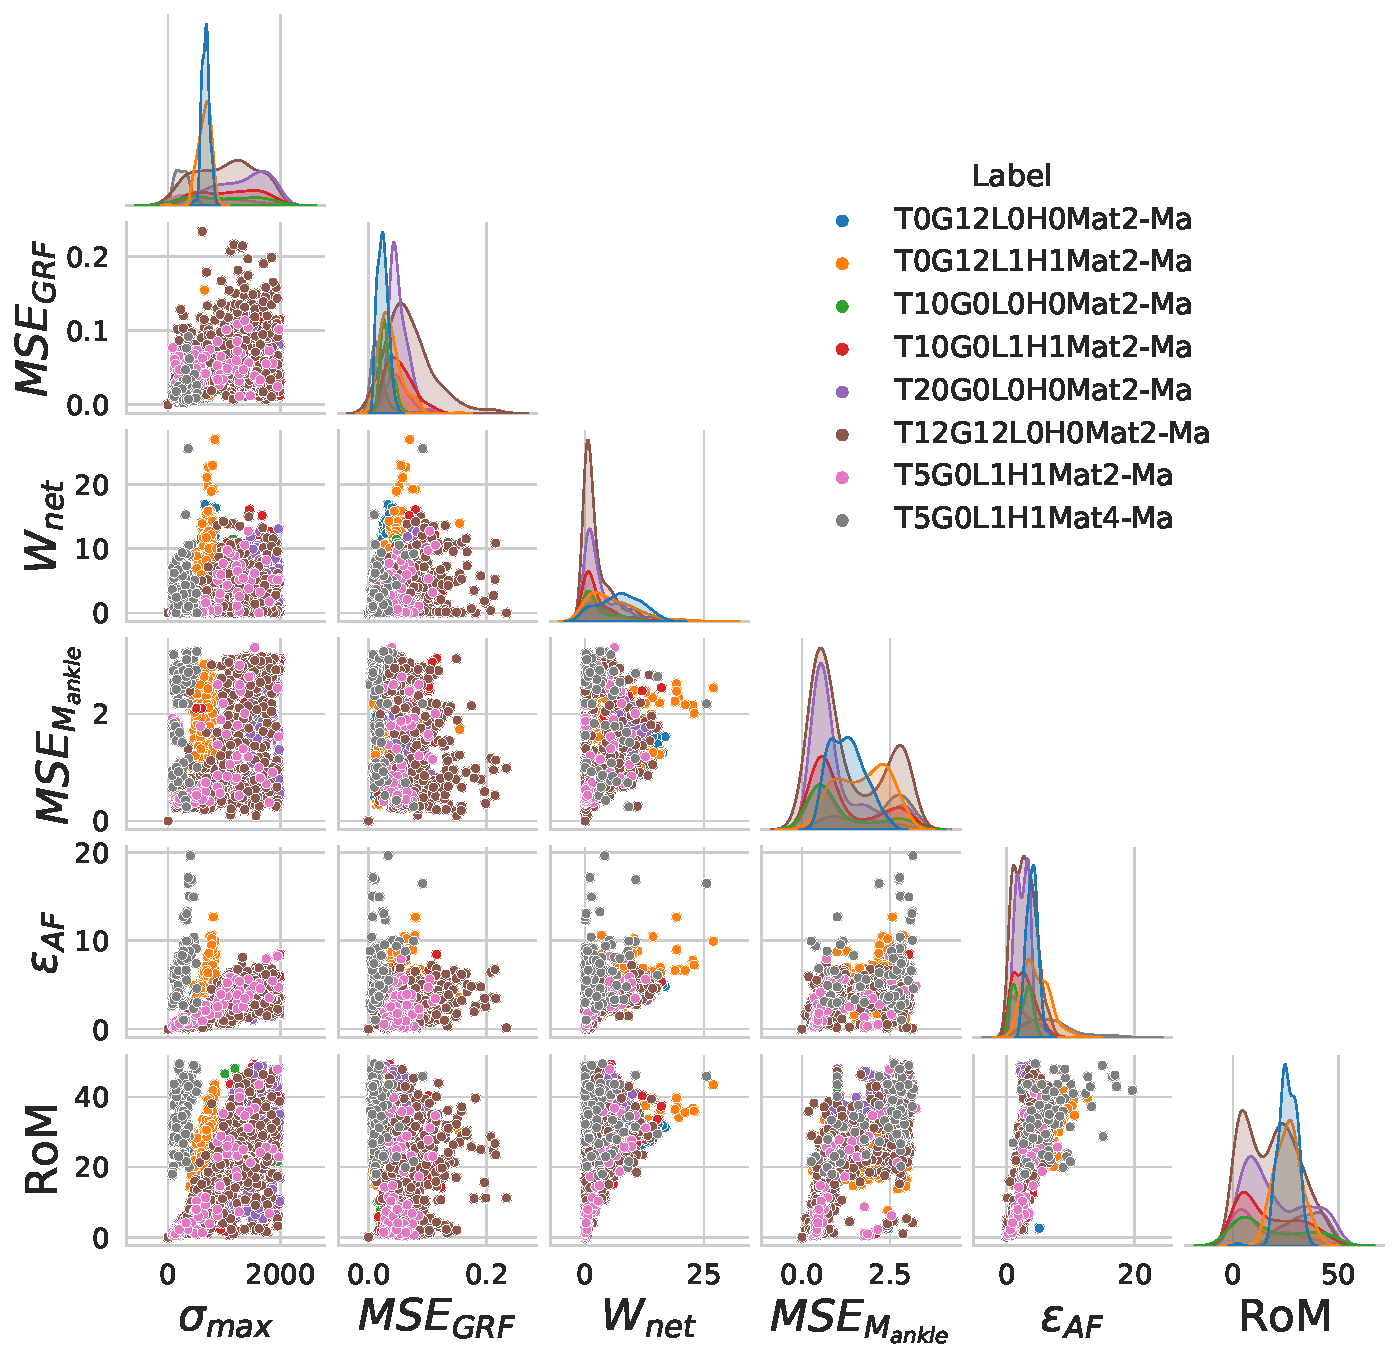
\includegraphics[scale=0.2]{Feathergraphics/PairPlotOutputsOfInterest.pdf}}
\caption{Visualization relationship among output variables of interest and their respective distribution in all experiments performed.}\label{fig:pairplot_LHS}.}
\end{figure}
\end{footnotesize}
\end{frame}


\begin{frame}{The validation and verification of the model.}
\begin{footnotesize}
\begin{figure}
\centerline{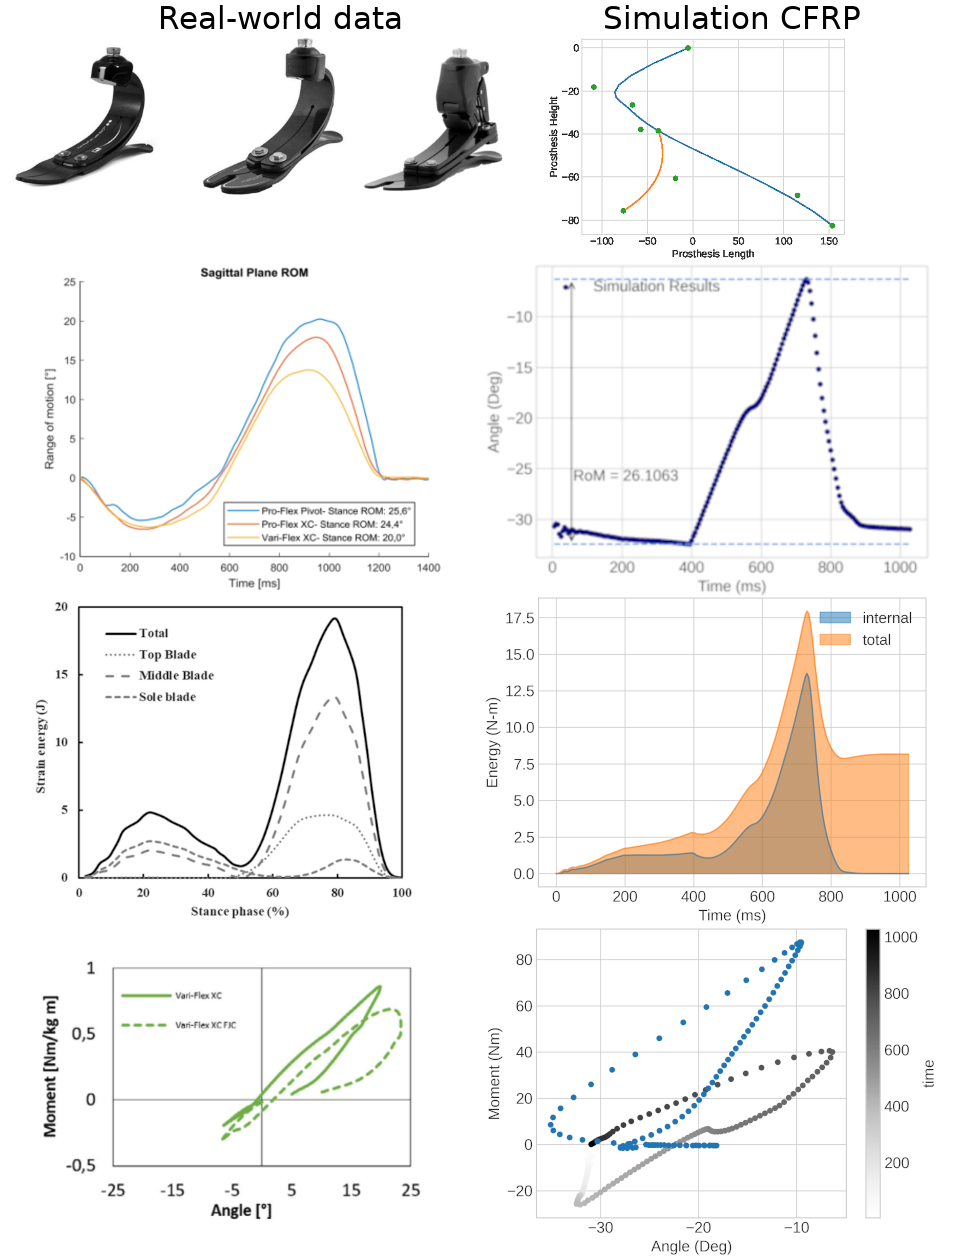
\includegraphics[scale=0.15]{Feathergraphics/comp_RoM_DJS.png}}
\caption{Ankle DJS, strain energy  and $RoM$ for three Pro-flex foot prostheses (left) \--- Images extracted from studies \cite{Tryggvason2020} and \cite{Lecomte2020} \--- and, simulation with the depicted shape and material CFRP (right). Consistent units are presented comparing $RoM$ and Strain Energy $\epsilon_{AF}$. For ankle DJS the simulation results are un-normalized as we do not count with the body mass.\label{fig:validation}}
\end{figure}
\end{footnotesize}
\end{frame}

%\begin{frame}{The pair plot of the SA}
%\begin{footnotesize}
%\begin{figure}
%\centerline{\includegraphics[scale=0.6]{Feathergraphics/
%\end{figure}
%\end{footnotesize}
%\end{frame}

\section{A surrogate model and bayesian optimization for the AF model.}

%\backupbegin
\begin{frame}[allowframebreaks]{Bibliografía}

%-------------------------------------------------------
\bibliographystyle{IEEEtran}
\tiny{\bibliography{Proposal.bib,patents.bib}}
\end{frame}
%\backupend

{\BiOM
\begin{frame}[plain,noframenumbering]
  \finalpage{Thank You!\\\emph{enprietop@unal.edu.co}}
\end{frame}}
% Appendix

\end{document}